%%%%%%%%%%%%%%%%%%%%%%%%%%%%%%%%%%%%%%%%%%%%%%%%%%%%%%%%%%%%%%%%%%%%%%%
%% Related Work
\section{Grundlagen}
\label{sec:basics}

Dieses Kapitel befasst sich mit den Grundlagen für die folgenden Kapitel. Es soll dem geneigten Leser Informationen zum Verständnis der Arbeit geben. Die anschließenden Unterkapitel beschreiben zunächst die verwendeten Mathematischen Ausdrücke und Bezeichner um die Lesbarkeit der späteren Formeln zu erleichtern. Nachfolgend wird die Middleware ROS genauer erläutert und unterschiedliche Funktionen sowie Einschränkungen aufgezeigt, die Auswirkungen auf die entwickelte Softwarearchitektur hatten. Darauf folgt eine Definition des Begriffs der Kinematik, welcher im späteren Verlauf der Arbeit für die Entwicklung der inversen Kinematik benötigt wird. Das abschließende Unterkapitel beschreibt die verwendete Hardware und den Laboraufbau im Detail. Weitere Informationen bezüglich der Robotik und grundlegender Mathematischer Begriffe sind im Buch "Robotics, Vision and Control" von Peter Corke zu entnehmen.

%%%%%%%%%%%%%%%%%%%%%%%%%%%%%%%%%%%%%%%%%%%%%%%%%%%%%%%%%%%%%%%%%%%%%%%
%% Related Work
\subsection{Nomenklatur}
\label{sec:basic-math}
    
  Die folgende Tabelle erläutert die genutzten mathematischen Symbole und orientiert sich an dem Buch \cite{Corke2011}. Von links nach rechts sind das Symbol, die Einheit und die Beschreibung gegeben. Einige Symbole werden mehrfach verwendet und haben je nach Kontext eine andere Bedeutung. Vektoren werden mit einem Bezeichner in \textbf{fett} gekennzeichnet.

  \begin{table}[h]%
  \begin{tabularx}{\columnwidth}{|l|l|X|}
  	\hline Symbol & Einheit & Beschreibung \\ 
  	\hline $T$ & s & Messintervall \\
 	\hline $T$ &  & homogene Transformation, $T \in SE(2)$ oder $SE(3)$ \\
 	\hline $^AT_B$ &  & homogene Transformation zur Darstellung von Koordinatensystem $ B $ betrachtet von Koordinatensystem $ A $. Koordinatensystem $ 0 $ bezeichnet das Weltkoordinatensystem und muss nicht explizit angegeben werden $^0T_B = T_B$(). Die inverse kann auf zwei Arten betrachtet werden: $(^AT_B)^{-1} = ^BT_A $ \\
 	\hline $\theta$ & rad & Winkel im Bogenmaß. Wenn nichts weiteres gegeben ist sind Winkel immer im \textbf{Bogenmaß} zu sehen. \\ 
 	\hline $ \pmb{\theta}$ & rad & Vektor von Winkel im Bogenmaß. \\ 
	\hline $\theta_r \theta_p \theta_y$ & rad & Roll-Pitch-Gear Winkel, beziehungsweise Rollen \\
 	\hline $\alpha$ & \textdegree & Winkel in Grad. Wenn nichts weiteres gegeben ist sind Winkel immer im \textbf{Bogenmaß} zu sehen. \\
 	\hline $v$ & m s$^{-1}$ & Geschwindigkeit. \\
 	\hline $\pmb{v}$ &  m s$^{-1}$  & Geschwindigkeitsvektor. Meist $\in \mathds{R}^3$. \\
 	\hline $\omega$ & rad s$^{-1}$ & Drehwinkel-Geschwindigkeit. \\
 	\hline $\pmb{\omega}$ &  rad s$^{-1}$  & Drehwinkel-Geschwindigkeitsvektor. Meist $\in \mathds{R}^3$. \\
 	\hline $\pmb{v}$ &  & Geschwindigkeit-Drehung (engl. Twist, Screw).  $\pmb{v} \in \mathds{R}^6$, $\pmb{v} = (v_x, v_y, v_z,\omega_x, \omega_y, \omega_z)$ \\
 	\hline X,Y,Z &   & Kartesische Koordinaten. \\
 	\hline $\xi$ &   & Abstrakte Darstellung einer 3-dimensionalen Kartesischen Pose  $\xi  \in \mathds{R}^6$ \\
 	\hline $^A\xi_B$ &   & Abstrakte Darstellung einer \textbf{relativen} 3-dimensionalen Kartesischen Pose, Pose $ B $ betrachtet von Pose $ A $ \\
	\hline $\oplus$ &   & Hintereinanderausführung (Addition) zweier Posen \\
	\hline $\ominus$ &   & Unärer Operator zur Invertierung von Posen \\
 	\hline
  \end{tabularx}
  \caption{Nomenklatur}
  \label{tab:nomenklatur}
  
    \end{table}%
  


%%%%%%%%%%%%%%%%%%%%%%%%%%%%%%%%%%%%%%%%%%%%%%%%%%%%%%%%%%%%%%%%%%%%%%%
%% Related Work
\subsection{ROS: Robotic Operating System}
\label{sec:basic-ros}
    
Das Robotic Operating System, kurz ROS, ist ein Middleware-Framework zur Steuerung und Verwaltung von Personal-Robotern. Es verwendet eine Paket und Node Struktur um einzelne Aktoren und Sensoren einzelner Robotersystem zu betreiben. Das ROS dient dabei als Abstraktionsebene für die Entwickler und versucht die Anwendungsebene von der Hardwareebene zu trennen. Das Framework wird am Robotikinstitut Willow Garage in Zusammenarbeit mit der Open Source Robotics Foundation entwickelt, stammt aber ursprünglich vom Stanford Artificial Intelligence Laboratory. Dort wurde 2007 im Rahmen des Stanford-AI-Robot-Projektes die Entwicklung aufgenommen. ROS ermöglicht während der Entwicklung und des Betriebs ein Cross-Plattform System, da es kompatible Versionen für Windows (experimentell), Linux und Mac OS X gibt. Außerdem steht ein Multi(programmier)sprachen System zur Verfügung. So ist es möglich, eigene Nodes mit C++, Python oder Java zu entwickeln \citep{quigley2009ros}. Neben den Standardkonzepten und -paketen gibt es eine Community, die eigene Pakete auf der ROS-Homepage zur Verfügung stellt. Die folgenden Abschnitte erläutern die ROS-Kernkonzepte, welche für die Entwicklung eingesetzt wurden. Als Grundlage für das komplette Kapitel wurde die Dokumentation von ROS genutzt.

\subsubsection{Packages und Nodes}

\textit{Packages} dienen der strukturellen Verwaltung aller Dateien im ROS-System. Nodes, Launch-Files, Services, Actions und Messages (siehe unten) sind immer an ihr Paket gebunden und können nur unter deren Namen erreicht werden. Für die Verlinkung und die Erreichbarkeit gebauter Pakete ist das ROS-interne Buildsystem \textit{Catkin} zuständig. Es benötigt ebenfalls den \textbf{eindeutigen} Package-Namen für den Build und Verwaltungsprozess. Neben den ROS-bezogenen Daten können in einem Paket aber auch ROS unabhängige APIs angelegt und verwaltet werden. So werden unter anderem einzelne Pakete für Treiber genutzt. Ein ROS-Paket folgt dem Goldilocks-Prinzip: Genug Funktionalität um nützlich zu sein, aber nicht zu viel, damit die Verwendbarkeit nicht zu komplex wird \citep{roswiki}.

Neben der strukturellen Verteilung gibt es auch die funktionale Trennung. Diese wird durch einzelne \textit{Nodes} erreicht. Jeder Node hat einen bestimmten Aufgabenbereich. Erst das Zusammenspiel mehrerer Nodes ergibt ein Robotersystem. So ist ein Node zum Beispiel für die Berechnung der inversen Kinematik zuständig, ein anderer für die Lokalisierung des Roboters im Raum und ein dritter für das User-Interface. Diese Verteilung der Funktionalitäten hat mehrere Vorteile. Da jeder Node in einem eigenen Prozess gestartet wird, ist das komplette System robuster. Jeder Node muss so entwickelt werden, dass er eigenständig weiterlaufen kann, auch wenn ein benötigter Node durch einen Fehler abgestürzt ist. Jeder Node wird mit einem systemweit einmaligen Namen aufgerufen unter dem er vom System erreicht und angezeigt werden kann. Nodes kommunizieren untereinander mit Hilfe von Topics (siehe \ref{sec:basic-ros-topics}). Soll ein ROS Node gestartet werden kann dieser mit Hilfe des ROS-Befehls aufgerufen werden \citep{roswiki}:

\begin{lstlisting}[language=bash]
rosrun <paket-name> <nodetype-name>
\end{lstlisting}

Der Paketname und der Nodetype sind erforderliche Felder. Darüber hinaus können Parameter angegeben werden, die für den Node notwendig sind. Eine weitere Möglichkeit einen und mehrere Nodes zu starten, ist ein Launchfile. In diesem können Nodes, Parameter und Argumente aufgelistet werden. Zu beachten ist jedoch, dass die Nodes in einer zufälligen Reihenfolge gestartet werden. Ein Launch-File kann mit folgendem Befehl gestartet werden \citep{roswiki}:

\begin{lstlisting}[language=bash]
roslaunch <paket-name> <launchfile-name>
\end{lstlisting}

Damit ein Node gestartet werden kann, muss vorher ein ROS-Master aktiv sein, mit dem sich der Node verbinden kann. Ist der Node verbunden kann er auf die Topics, Services, Actions und den Parameter-Server des Master zugreifen \citep{roswiki}.

\subsubsection{Master und Parameter-Server}
Der ROS Master ist ein zentraler Dienst für ganze System. Er beinhaltet einen Namen- und Registrierungs-Service an dem sich andere Nodes, auch Services, anmelden können. Der Master wird benötigt, damit die Nodes sich gegenseitig im System verbinden können. Der Nachrichten-Transport geht nicht direkt über den Master. Dieser verbindet nur die beiden Nodes, welche anschließend via einer Peer-to-Peer Verbindung kommunizieren \citep{roswiki}. In Abbildung \ref{fig:basic-ros-masternode} ist eine solche Verbindung dargestellt.

 \begin{figure}[h]
 	\centering
 	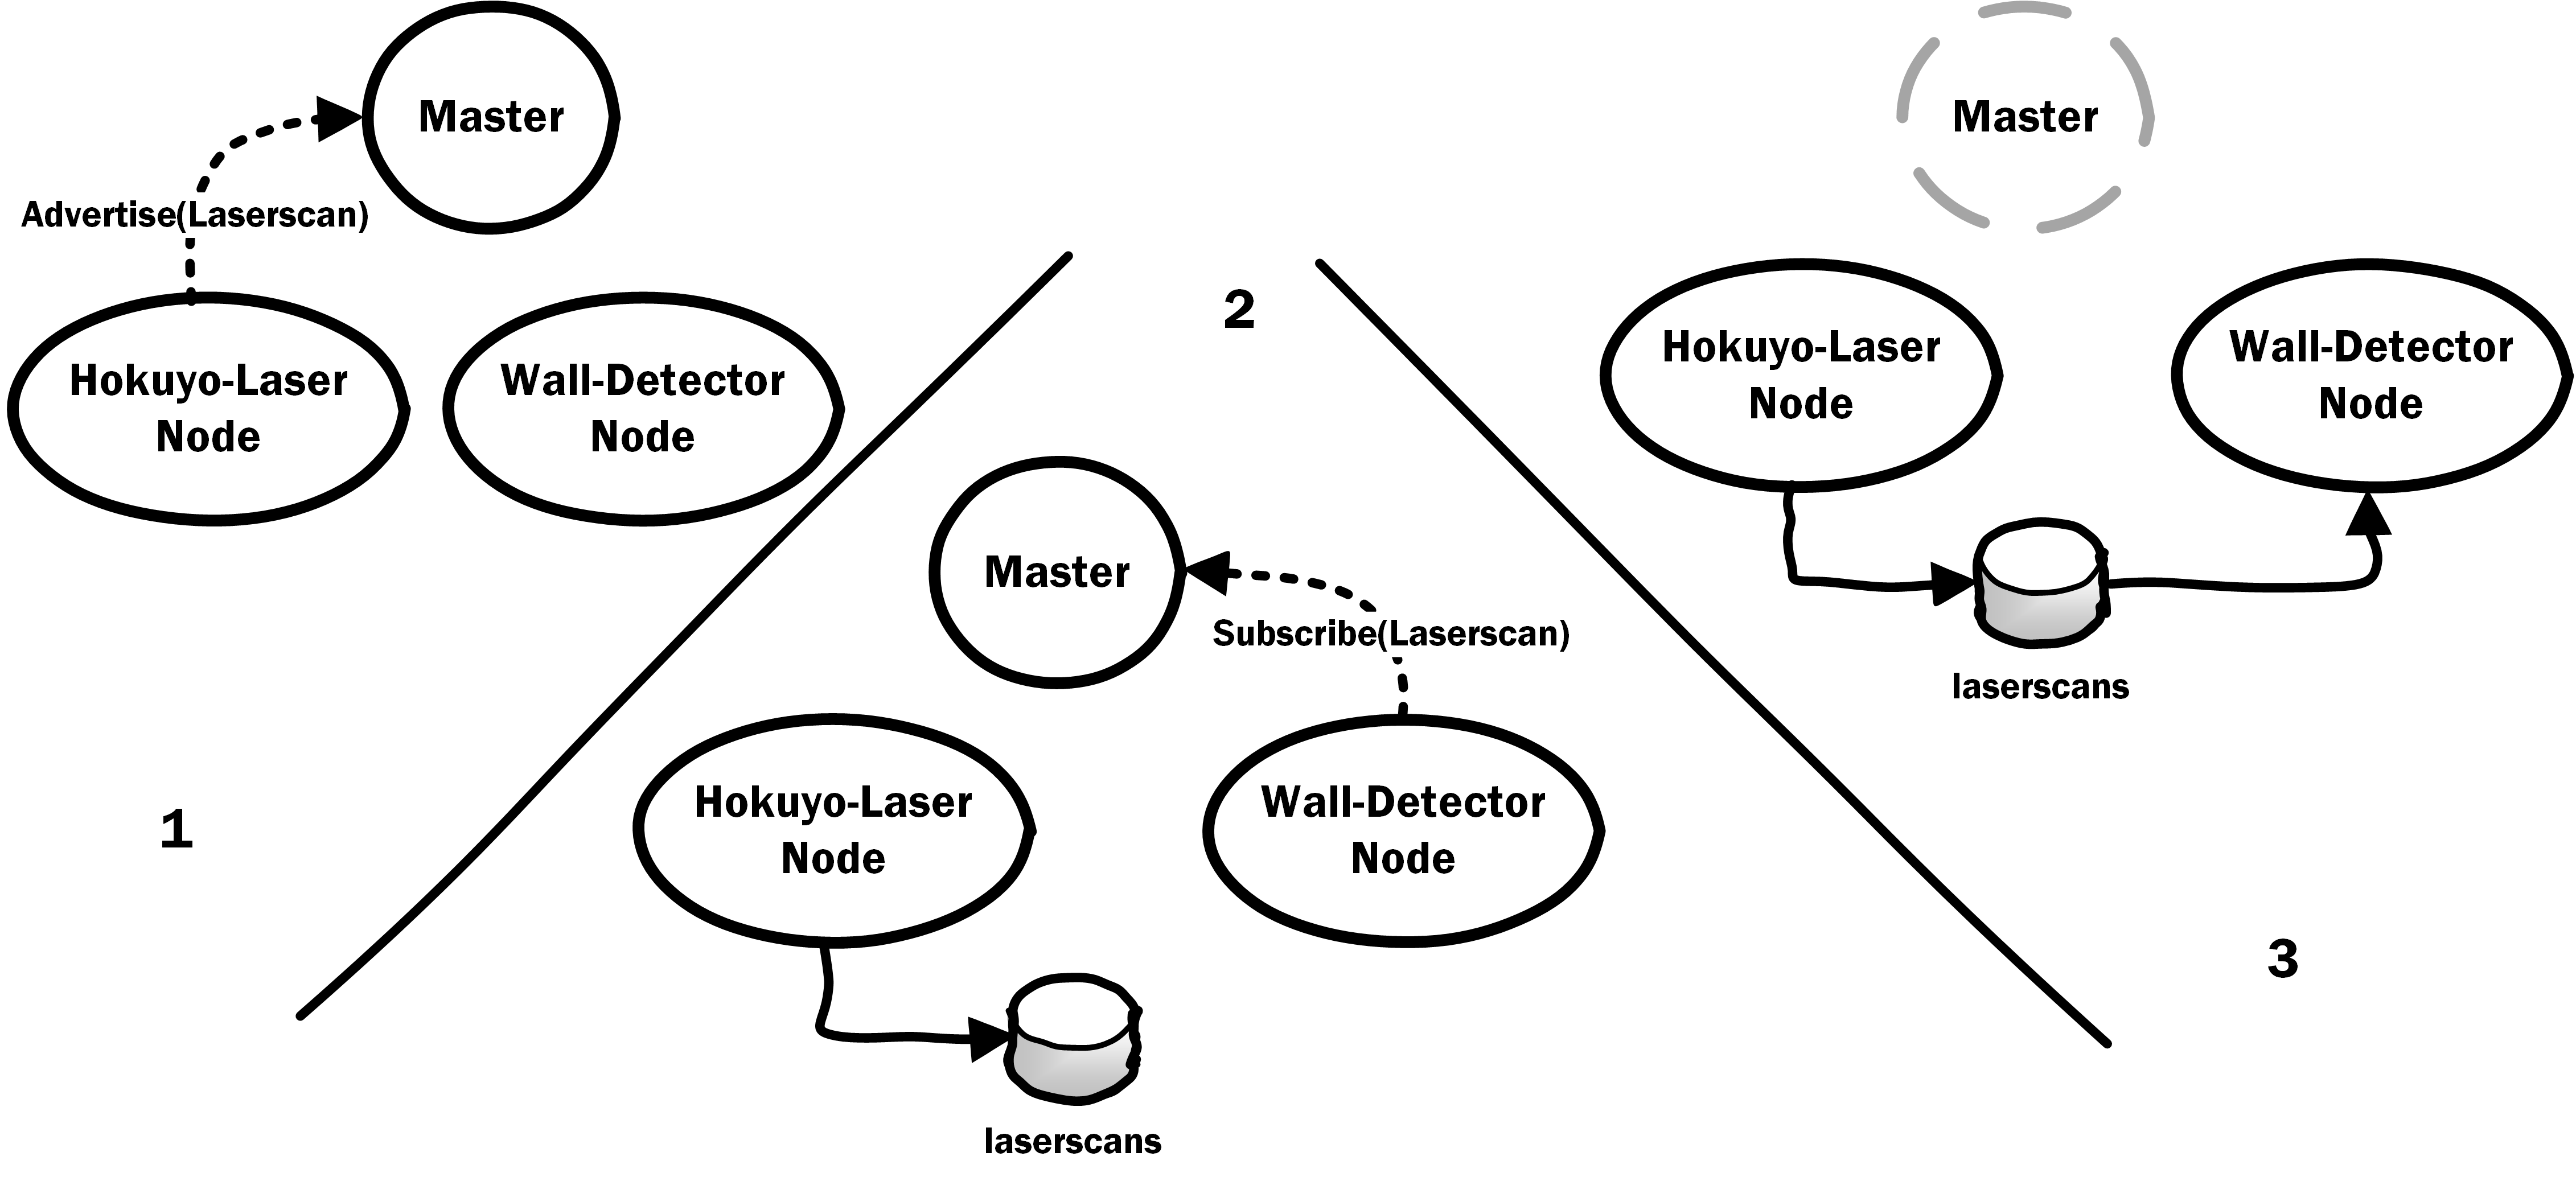
\includegraphics[scale=0.8]{fig/masternode}   
 	\caption[Master-Service]{Master-Service: (1) Der Hokuyo-Laser-Node meldet sich beim Master an, dass er Laserscans zur Verfügung stellt. (2) Der Laser-Node stellt seine Daten zur Verfügung und der Wall-Detector meldet sich beim Master, dass er Laserscans benötigt. Der Master stellt die Verbindungsinformationen bereit und zieht sich dann zurück (graue Markierung). (3) Die Verbindung zwischen Laser-Node und Detector-Node ist hergestellt.}
 	\label{fig:basic-ros-masternode}
 \end{figure}
 
 Dieses Verfahren reduziert die Netzwerklast stark im Vergleich zu einem Broadcasting-Verfahren. Eigene Tests im Rahmen dieser Arbeit zeigten, dass der Kamera-Node \textit{openni2} ein Netzwerk mit den berechneten 3D-Punktwolken vollständig auslastet. Dabei wurde die Punktwolke auf einer physikalischen Maschine  erzeugt und auf eine zweite Maschine via WLAN übertragen. Die Verzögerung der Wolken war dabei mit über fünf Sekunden im Schnitt sehr hoch und wurde höher, je länger die Übertragung dauerte. Eine Lösung (siehe \ref{fig:basic-ros-masternet}) bietet die Vorverarbeitung der Daten auf der Maschine. Dabei werden nur noch die gefilterten Daten übertragen, sowie die Übertragungsrate reduziert. Dadurch ist die Übertragung der Daten unkritisch. Nun gingen nur noch die Verbindungsdaten zwischen Nodes und Master und die reduzierte Datenmenge über das Netzwerk.
 
 \begin{figure}[h]
 	\centering
 	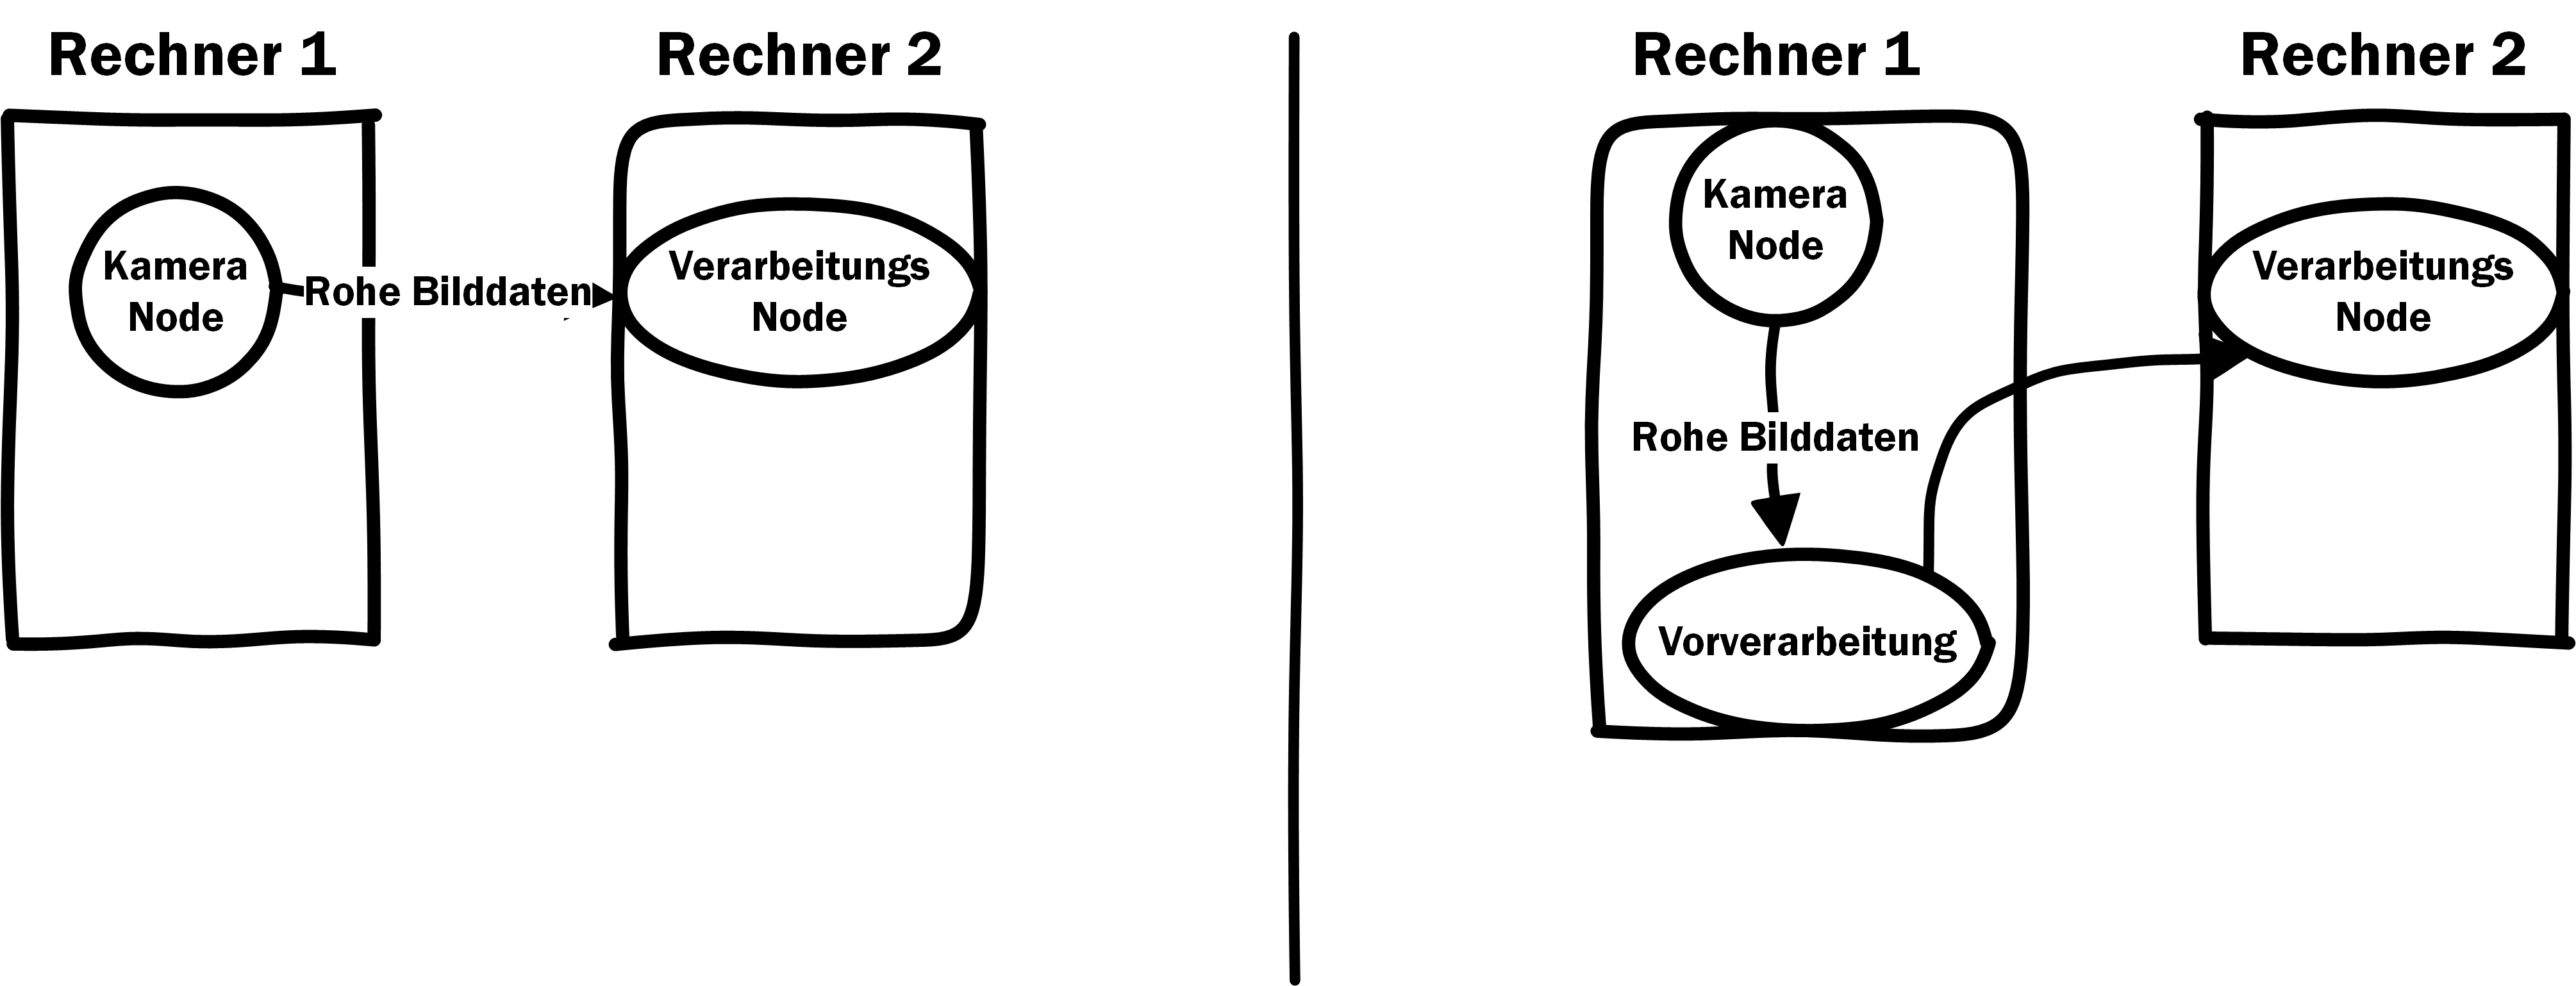
\includegraphics[scale=0.8]{fig/masternet}   
 	\caption[Netzwerk Entlastung durch Peer-to-Peer Verbindungen]{Netzwerk Entlastung durch Peer-to-Peer Verbindungen. Links: ohne Datenvorverarbeitung, Rechts: mit Datenvorverarbeitung.}
 	\label{fig:basic-ros-masternet}
 \end{figure}
 
 Neben dem Namens-Service verwaltet der ROS-Master auch den Parameter-Server. Dieser besteht aus einer großen Key-Value-Map, dem Wörterbuch. Dieses kann global erreicht werden. Nodes haben so die Möglichkeit, vordefinierte Daten zu lesen oder selber welche zu schreiben. So können Sensoren oder Aktoren kalibriert und konfiguriert werden. Der Zugriff auf diese Daten hat keine hohe Performance. Er ist für einen statischen Zugriff gedacht und kann mit einer Baum-Struktur geordnet werden, so lassen sich zusammenhängende Daten mit einer Abfrage am Server abrufen \citep{roswiki}.

\subsubsection{Topics und Messages}
\label{sec:basic-ros-topics}

ROS bietet für die Kommunikation zwischen Nodes ein \textit{Topic}-System. Jeder Topic entspricht dabei einem benannten Bus, auf welchen anonyme \textit{Publisher} und \textit{Subscriber} zugreifen können. Die Daten können dabei als TCP-Pakete (TCPROS) oder als UDP-Pakete (UDPROS) gesendet werden. Ein Topic besitzt einen eindeutigen Namen im System und einen eindeutigen Typen, der anhand des übersendeten Message-Typen definiert wird. Jede Topic kann nur einen Message-Typen versenden. Dieser Type ist nicht im Master bekannt, jedoch können sich Subscriber nur mit dem entsprechenden Typen anbinden. Die Anzahl der Subscriber und Publisher für einen Topic ist nur durch die Systemleistung beschränkt \citep{roswiki}. In Abbildung \ref{fig:basic-ros-topic} ist ein solcher Topic dargestellt.

\begin{figure}[h]
	\centering
	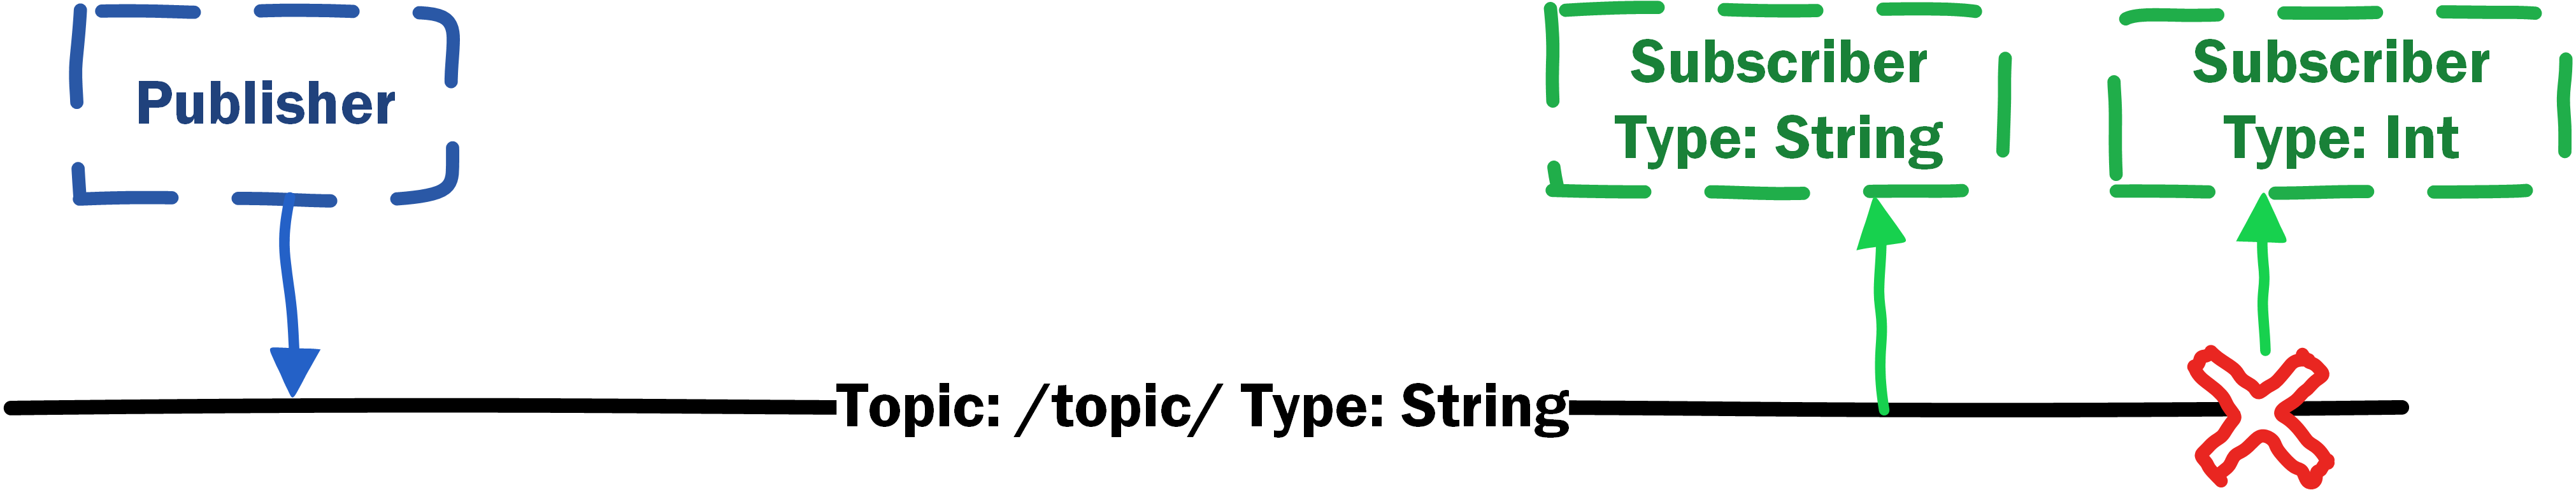
\includegraphics[scale=0.8]{fig/topic}   
	\caption[Topic Beispiel]{Beispiel für ein Topic mit dem Namen /topic/ und dem Type String. Ein Publisher schreibt Daten in den Bus, ein Subscriber liest diese aus. Die Verbindung eines zweiten Subscribers schlägt auf Grund des falschen Types fehl.}
	\label{fig:basic-ros-topic}
\end{figure}

Publisher veröffentlichen ihre Daten in den Bus und haben nur einen schreibenden Zugriff. Sie bekommen kein Feedback, an wen die Daten gesendet worden sind, oder ob die Daten überhaupt empfangen worden sind. Der erste Publisher, der sich auf einem Topic verbindet, gibt den Typen vor \citep{roswiki}.

Subscriber lesen die Daten vom Bus und geben sie für die Weiterverarbeitung weiter. Sie bekommen normalerweise keine Informationen über den Absender der Daten. Subscriber können sich nur bei einem Topic registrieren, wenn der Message-Type stimmt \citep{roswiki}.

Subscriber und Publisher haben jeweils eigene Cache-Systeme, die Nachrichten vor- oder zurückhalten können. Ein Topic ist ein einfachgerichteter Streaming-Dienst. Da in einem Roboter-System auch Remote-Procedure-Calls benötigt werden, um zum Beispiel Antworten auf Anfragen zu erhalten oder synchronisierte Aufgaben zu erledigen, wurde das Service-Paket als weiteres Kernkonzept angelegt \citep{roswiki}.

\subsubsection{Services}

\textit{Services} ermöglichen es einen Remote-Procedure-Call Node-übergreifend durchzuführen. Dazu muss Node A seinen Service am Master registriert haben und einen Service-Server gestartet haben. Node B kann nun mit einem Service-Client auf den registrierten Service zugreifen und eine Anfrage starten. Während die Anfrage verarbeitet wird, kann Node B nun je nach Anforderung blockieren oder weiter arbeiten. Node A verarbeitet nun die Anfrage und antwortet Node B mit dem Ergebnis. Der Service selbst, sowie die Parameter und die Rückgabewerte, sind für jeden Service eindeutig und werden vorher über zwei Messages, eine für die Request und eine für die Response, festgelegt. Analog zu den Topics werden Services am Master mit einem eindeutigen Namen angemeldet, unter dem sie erreichbar sind. Dies ermöglicht auch einen einfachen Austausch von verschiedenen Implementierungen \citep{roswiki}.

\subsubsection{Action-Lib}
\label{sec:basic-ros-action}
Ein aktiver Service schickt erst eine Rückmeldung an den Aufrufer, wenn er seine Aufgabe erledigt hat. Um auch einen Zwischenstand schicken zu können, wurde die Action-Lib eingeführt. Dieses Paket ist eigentlich keine Entwicklung der ROS-Entwickler sondern ein Community-Package. Inzwischen wurde es aber von der OSR-Foundation übernommen und als eins der Kernkonzepte eingestuft \citep{roswiki}.

Analog zu den Services besitzt auch die Action-Lib einen Server- und einen Client-Teil. Der Client fordert vom Server eine Aktion an, dabei übergibt er ein \textit{Goal}. Dieses beinhaltet die benötigten Parameter für den Server. Der Server arbeitet die Anfrage ab, dabei kann er auch \textit{Feedback} zurückschicken. Dies können mögliche Zwischenergebnisse oder Fortschrittsmarken sein. Ist die Anfrage abgearbeitet, schickt der Server ein \textit{Result} an den Client zurück. Wie auch beim Service ist die Art der Aktion eindeutig. Die Anzahl der Parameter bei Goal, Feedback und Result sind fest definiert und können zur Laufzeit nicht geändert werden \citep{roswiki}.
%%%%%%%%%%%%%%%%%%%%%%%%%%%%%%%%%%%%%%%%%%%%%%%%%%%%%%%%%%%%%%%%%%%%%%%
%% Related Work
\subsection{Kinematik }
\label{sec:basics-ik}
    
Dieses Unterkapitel befasst sich mit dem Begriff der Kinematik und den dazu gehörigen Begriffen des Mechanismus und der inversen Kinematik. Außerdem werden einige mathematische Lösungswege für verschiedene Probleme innerhalb der genannten Themen genannt.

\subsubsection{Mechanismus}

Ein Mechanismus ist der Grundbegriff von beweglichen Körper. Dabei wird zwischen \textit{Gliedern} (engl. Link, $L$ = Set of Links) und \textit{Gelenken} (engl. Joint, $J$ = Set of Joints) unterschieden. Glieder sind die starren Körper eines Mechanismus und sind durch Gelenke miteinander verbunden. Ein Glied ist nicht auf ein Gelenk beschränkt, sondern kann mehrere haben ($N_{joint} \in \mathds{N}_0$). Auch die Verbindung zwischen zwei Gliedern kann durch mehrere  Gelenke realisiert sein. Ein Gelenk wiederum ist auf genau zwei Glieder beschränkt  ($N_{link} = 2$) und ermöglicht so eine eingeschränkte relative Bewegung zueinander. Gelenke werden nicht als eigenständige physikalische Körper gesehen. Gelenkhälften, zum Beispiel die Schenkel eines Kippscharniers, werden als Bestandteil des damit verbundenen Gliedes betrachtet. Die folgenden Definitionen sind als Denavit–Hartenberg Parameter bekannt \citep{Corke2011}.

Glieder können mit zwei Parametern definiert werden, der Länge $a$ und der Verdrehung $\alpha$:

\begin{displaymath}
	l_i \in L \\
\end{displaymath}

\begin{equation}
a_i =  \text{Länge von } l_i
\end{equation}

\begin{equation}
\alpha_i =  \text{Verdrehung von } l_i 
\end{equation}

Gelenke werden ebenfalls mit zwei Parametern definiert. Der Gelenk-Offset beschreibt den Abstand zwischen den zwei Gliedern eines Gelenks auf der Gelenkachse. Der Gelenkwinkel beschreibt die Rotation zwischen den beiden verbundenen Glieder im Bezug zur Gelenkachse\citep{Corke2011}.  Zur Veranschaulichung dieser Nomenklatur ist die Abbildung \ref{fig:ik-dh} vorhanden. Dabei sind die Parameter in rot dargestellt. Außerdem werden die einzelnen Koordinatensysteme der Gelenke gezeigt.

\begin{displaymath}
j_i \in J \\
\end{displaymath}

\begin{equation}
d_i =  \text{Gelenk-Offset von } j_i
\end{equation}

\begin{equation}
\theta_i =  \text{Gelenkwinkel von } j_i 
\end{equation}

\begin{figure}[H]
	\centering
	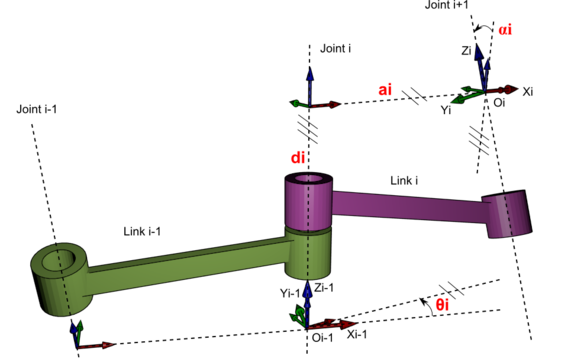
\includegraphics[width=0.8\textwidth]{fig/dh}   
	\caption[Darstellung Denavit–Hartenberg Parameter]{Darstellung Denavit–Hartenberg Parameter. Bildquelle \cite{wiki}}
	\label{fig:ik-dh}
\end{figure}

\subsubsection{Kinematik}
\label{sec:basics-ik-k}

Die \textit{Kinematik} eines Mechanismus beschreibt die Bewegungsmöglichkeiten der Glieder relativ zueinander. Es wird dabei abstrahiert, ob ein Gelenk motorisch angetrieben oder passiv bewegt wird. Die Kinematik betrachtet bei der Bewegung auftretende \textit{Geschwindigkeiten} und \textit{Beschleunigungen}. Auftretende Kräfte werden nicht in der Kinematik, sondern in der \textit{Dynamik} untersucht. Zentrale Aspekte dabei sind die Trägheits- und Schwerkraft.

Die \textit{Kinematische Kette} beschreibt den Aufbau eines speziellen Mechanismus. Dabei ist die Anzahl der Gelenke pro Glied auf maximal 2 beschränkt ($N_{joint} <= 2$). Besitzt jedes Glied genau zwei Gelenke gilt die Kette als geschlossen, ansonsten als offen.

\begin{equation}
	 \text{Kinematische Kette} = 
	\begin{cases}
		geschlossen & \forall l \in L | l_{joints} = 2 \\
		offen & \text{für Rest} \\
	\end{cases}
\end{equation}

Für diese Arbeit ist nur die offene Kette interessant, da die Manipulatoren der meisten Roboter an beiden Enden (Base und End-Effektor) frei sind. Dadurch ergibt sich für $N_{link} = N_{joint} + 1$. Typischerweise wird das erste Gelenk mit dem Index 1 versehen und das erste Glied mit dem Index 0. Glied 0 ist die \textit{Base} des Manipulators und Glied N beinhaltet den\textit{ End-Effektor}. Aus der Bezeichnung ergibt sich, dass Gelenk j die Glieder j-1 und j mit einander verbindet und das Glied j bewegt \citep{Corke2011}. 

Die Transformation eines Glied-Koordinatensystems {j-1} zu Glied {j} wird durch elementare Rotation und Translation beschrieben (siehe auch Abbildung \ref{fig:ik-dh}):

\begin{equation}
^{j-1}A_{j}(\theta_j,d_j,a_j,\alpha_j) = T_{Rz}(\theta_j)T_{z}(d_j)T_{x}(a_j)T_{Rx}(\alpha_j)
\label{f:basics-ik-k}
\end{equation}


Durch die Vereinigung der einzelnen Matrizen ergibt sich \cite{Corke2011}:
\begin{equation}
^{j-1}A_{j}(\theta_j,d_j,a_j,\alpha_j) = 
\begin{pmatrix}
cos \theta_j & -sin \theta_j cos \alpha_j & sin \theta_j sin \alpha_j  & a_j cos \theta_j\\
sin \theta_j & cos \theta_j cos \alpha_j & -cos \theta_j sin \alpha_j  & a_j sin\theta_j\\
0 			&sin \alpha_j 				& cos \alpha_j  & d_j\\
0 & 0 & 0& 1\\
\end{pmatrix}
\end{equation}

\subsubsection{Forward Kinematics}

Die Vorwärts-Kinematik (engl. Forward Kinematic) beschreibt die "vorwärts"  Rechnung der Kinematik. Aus den gegebenen Gelenk-Informationen wird die Pose des End-Effectors $\xi_E$ berechnet. Hier reichen die Daten für den Gelenkwinkel $\theta_j$ bei Drehgelenken und für den Winkel-Offset $d_j$ bei Schiebe-/ Schubgelenken, da die restlichen Werte für den Mechanismus als konstant angesehen werden können. Die Forward Kinematic wird häufig als Funktion $K$ angegeben \citep{Corke2011}.

\begin{equation}
\xi_E = K(\textbf{q})
\label{f1}
\end{equation}

$q$ entspricht dabei der aktuellen Gelenk-Konfiguration und $\xi_E$ der Pose des End-Effectors. Durch die Kombination der Transformation aus Gleichung \ref{f:basics-ik-k} ergibt sich für einen Manipulator mit N-Gelenken  \cite{Corke2011}. Dies wird benötigt, um die aktuelle Pose des End-Effektors für den Roboter zu berechnen. In dem Anwendungsszenario für diese Arbeit wird dies unter anderem für Positionsüberprüfungen und Kollisionskontrollen, aber auch für die Übergabe benötigt.

\begin{equation}
\xi_E \sim \: ^0T_E =\: ^0A_1\:^1A_2 \:\dots\:^{N-1}A_N
\end{equation}

\subsubsection{Inverse Kinematik}

Die Inverse Kinematik berechnet die Inverse der Forward-Kinematic. Sie bestimmt die möglichen Gelenk-Konfigurationen $\textbf{q}$ für eine Zielpose. Im Gegensatz zur Forward-Kinematic ist die Inverse Kinematik nicht eindeutig. Eine einfache Veranschaulichung kann man am menschlichen Körper sehen. Fixiert man das Handgelenk an einer Position kann man den Ellenbogen in verschiedene Positionen bewegen, ohne die Position der Schulter zu ändern. Für die Inverse Kinematik ergibt sich folgende Funktion für eine beliebige Pose $\xi$ \citep{Corke2011}:


\begin{equation}
\textbf{q} = K^{-1}(\xi)
\label{f2}
\end{equation}

Aus Gleichung \ref{f1} und \ref{f2} ergibt sich auf Grund der Eindeutigkeit:

\begin{displaymath}
\xi = K(K^{-1}(\xi))
\end{displaymath}

Aber \textbf{nicht}
\begin{displaymath}
\textbf{q} = K^{-1}(K(\textbf{q}))
\end{displaymath}

Um eine Inverse Kinematik zu lösen gibt es drei Methoden: geometrisch (analytisch), numerisch und heuristisch \citep{danielasteidl2011}.

Die geometrische Lösung nutzt die einfache geometrische Abstraktion des Mechanismus und versucht diesen mit trigonometrischen Funktionen abzubilden. Damit auch hier mehrere Lösungen bestimmt werden können, werden verschiedene Konfigurationen für bestimmte Abstraktionsmodelle geschaffen und alle Konfigurationen berechnet. Am Beispiel des Menschen wären mögliche Konfigurationen: \"Ellenbogen oben\" oder \"Ellenbogen unten\". Bei der Verwendung der trigonometrischen Funktionen muss beachtet werden, dass die Umkehrfunktionen in bestimmten Bereichen nicht eindeutig, ungenau oder gar nicht definiert sind. Empfohlen wird dafür die Verwendung von atan2, der in den meisten Programmiersprachen vorhanden ist. Diese Methodik funktioniert nur für einfache Mechanismen bei denen möglichst alle Gelenke die selben Achsen haben.

Die numerische Lösung versucht durch Iterationen eine Näherung an die gewünschte End-Pose zu erreichen. Das ganze fällt in die Thematik der Optimierung. Für die numerische Lösung gibt es unterschiedliche Algorithmen. Dazu gehören Jacobian-Transpose, Pseudo-Inverse und Damped-Least-Square. Die numerischen Lösungen sind im Vergleich zur analytischen langsamer und ungenauer, jedoch lassen sich mit ihr größere und komplexere Manipulatoren berechnen \citep{danielasteidl2011}.

Die heuristischen Lösungen nutzen abstrakte Bezüge und Vorhersagen für Veränderungen der Ziel-Pose im Bezug zur Gelenk-Konfiguration um mögliche Konfigurationen zu bestimmen. Eine anschließende Güteberechnung (zum Beispiel euklidische Distanz) gibt an, ob eine Konfiguration verworfen oder angenommen wird. Wie für die numerische Lösung gibt es auch bei der heuristischen Lösung mehrere Algorithmen. Diese sind unter anderem Cyclic Coordinate Descent und Lagrange-Multiplier \citep{danielasteidl2011}.

%Weitere Informationen zu den verschiedenen Algorithmen und ein Vergleich zwischen finden sich im Anhang

%%%%%%%%%%%%%%%%%%%%%%%%%%%%%%%%%%%%%%%%%%%%%%%%%%%%%%%%%%%%%%%%%%%%%%%
%% Related Work
\section{Laboraufbau}
\label{sec:basic-aufbau}
    
Dieses Kapitel befasst sich mit dem Aufbau der Versuchsanlage und der verwendeten Hardware. Dabei werden die Aspekte des räumlichen Aufbau genauso betrachtet wie die Netzwerkinfrastruktur und die genutzten Roboter und Sensoren.



\subsection{Aufbau Teststand}

 \begin{figure}[h]
 	\centering
 	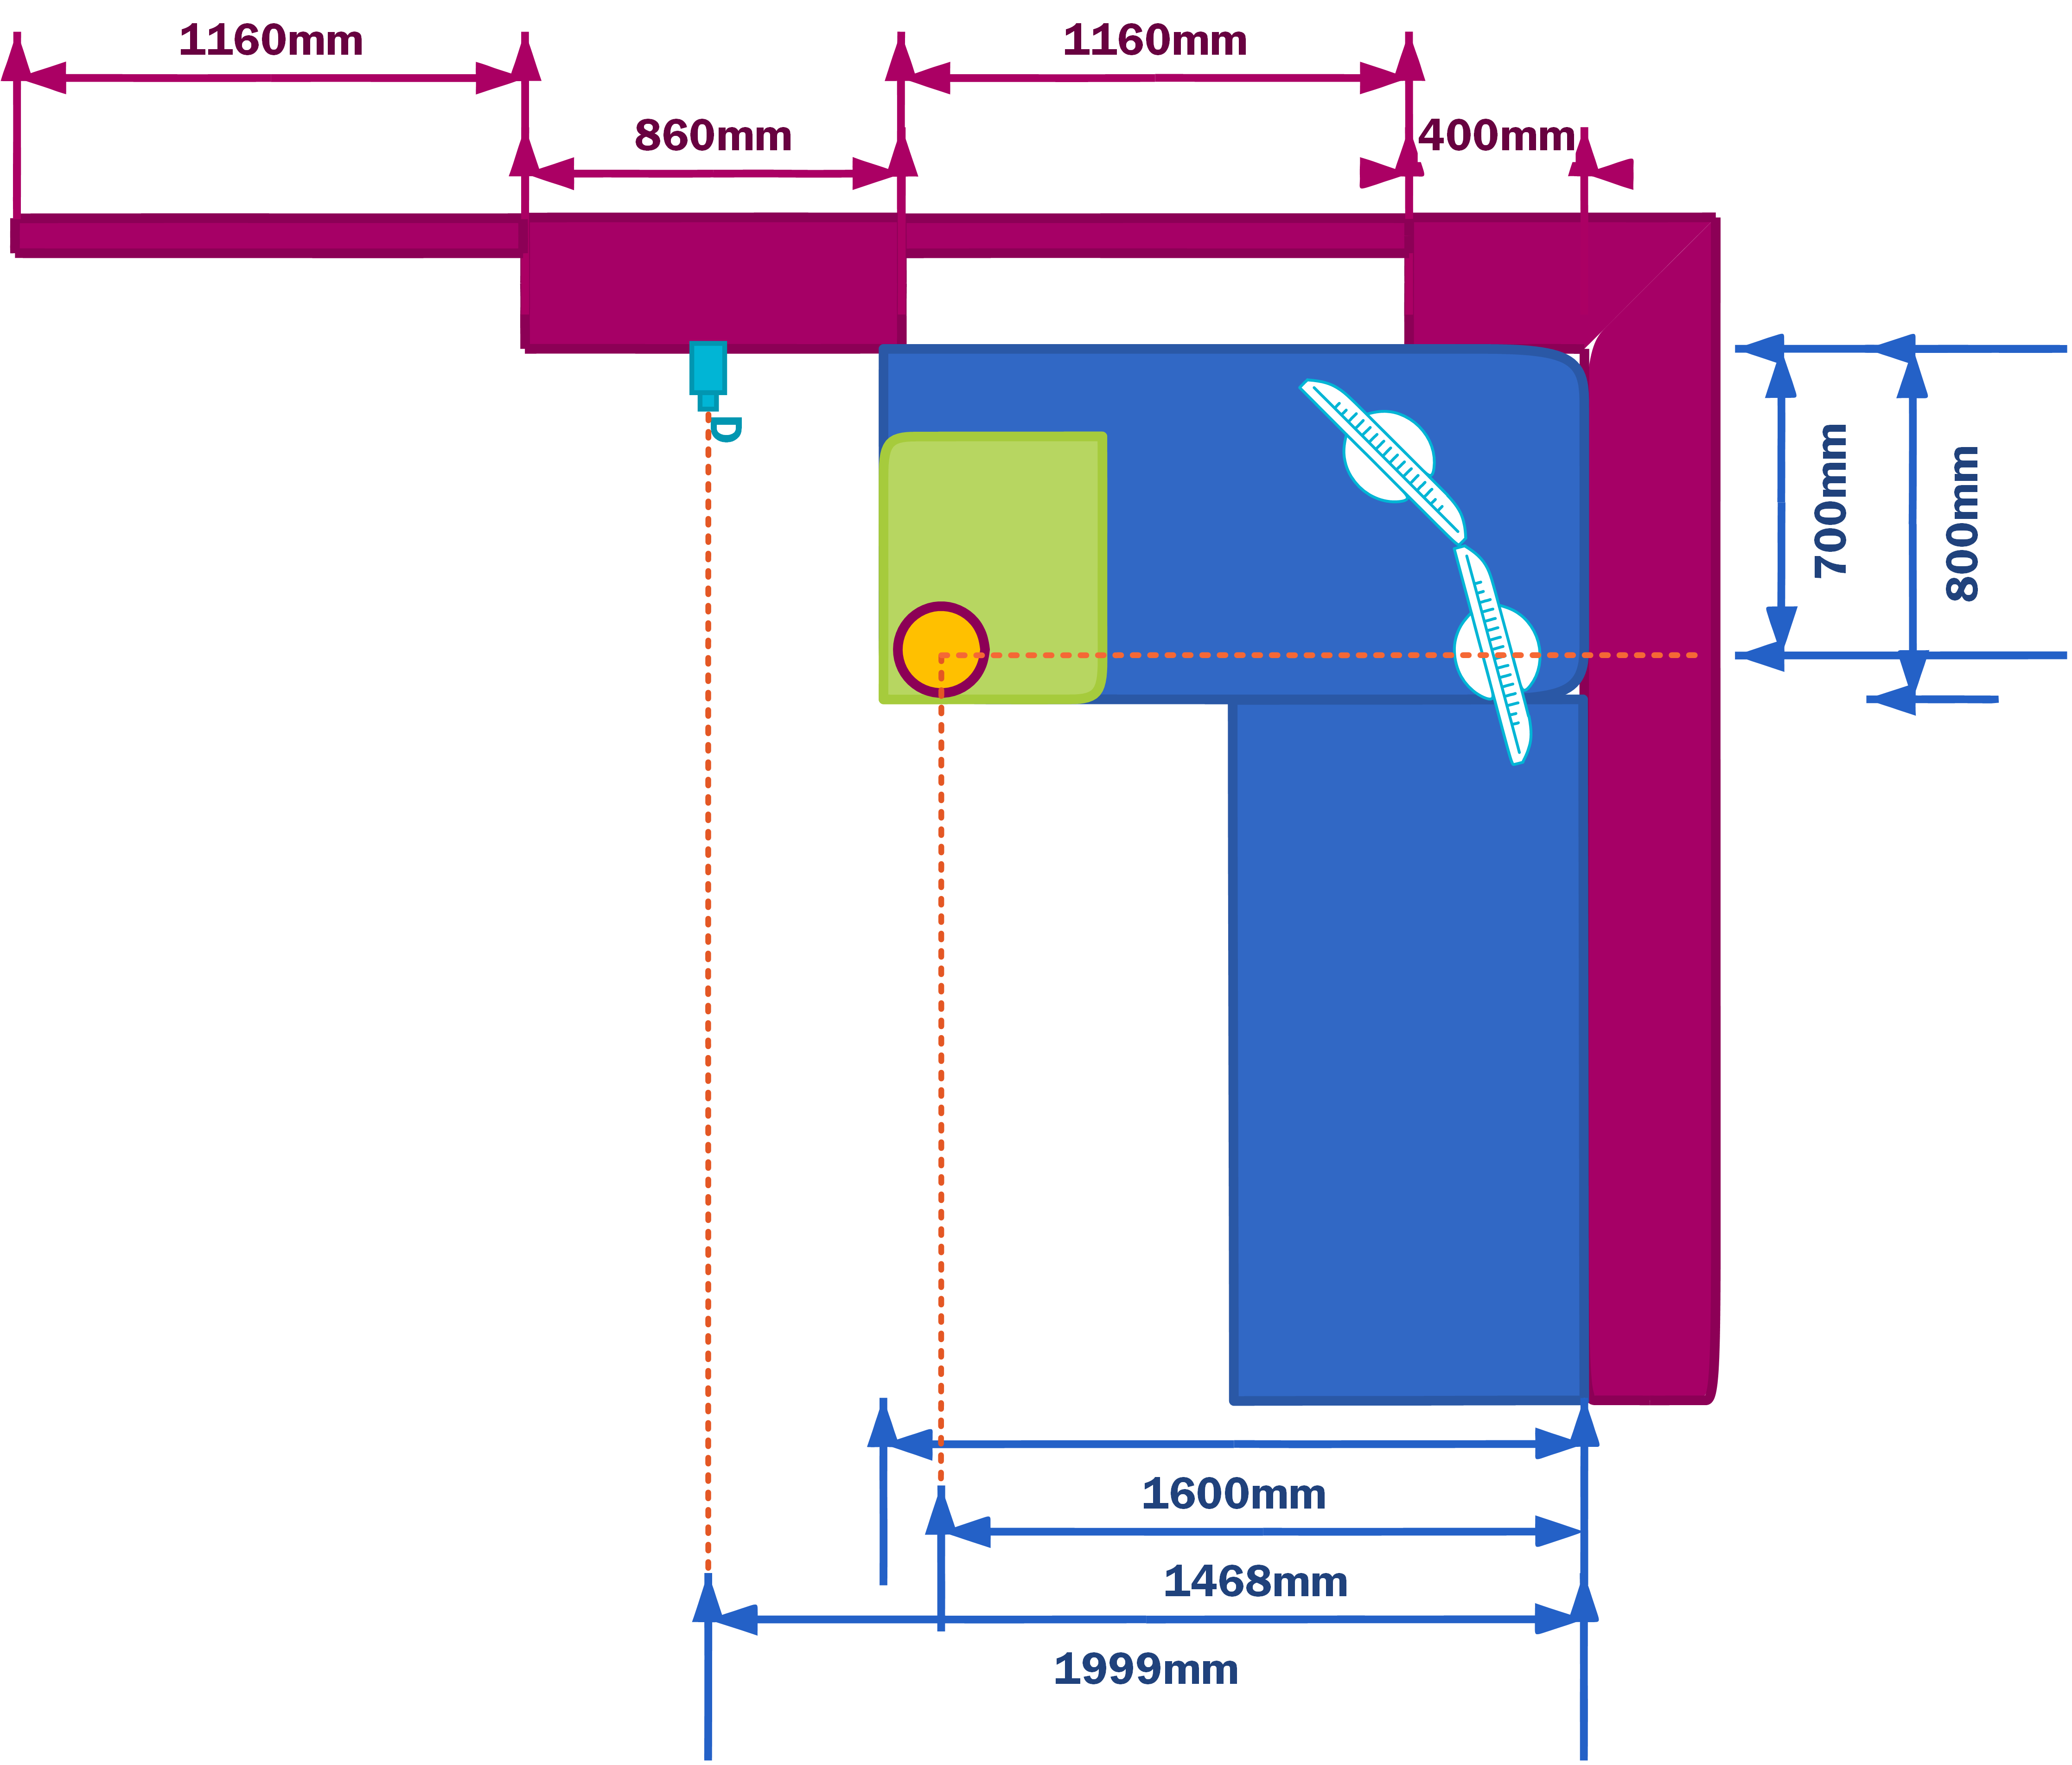
\includegraphics[scale=0.8]{fig/ZeichnungRaum}   
 	\caption[Aufbau Teststand: Draufsicht]{Der Aufbau der Testanlage als Draufsicht.}
 	\label{fig:basic-aufbau-teststand}
 \end{figure}
 
 
  \begin{figure}[h]
  	\centering
  	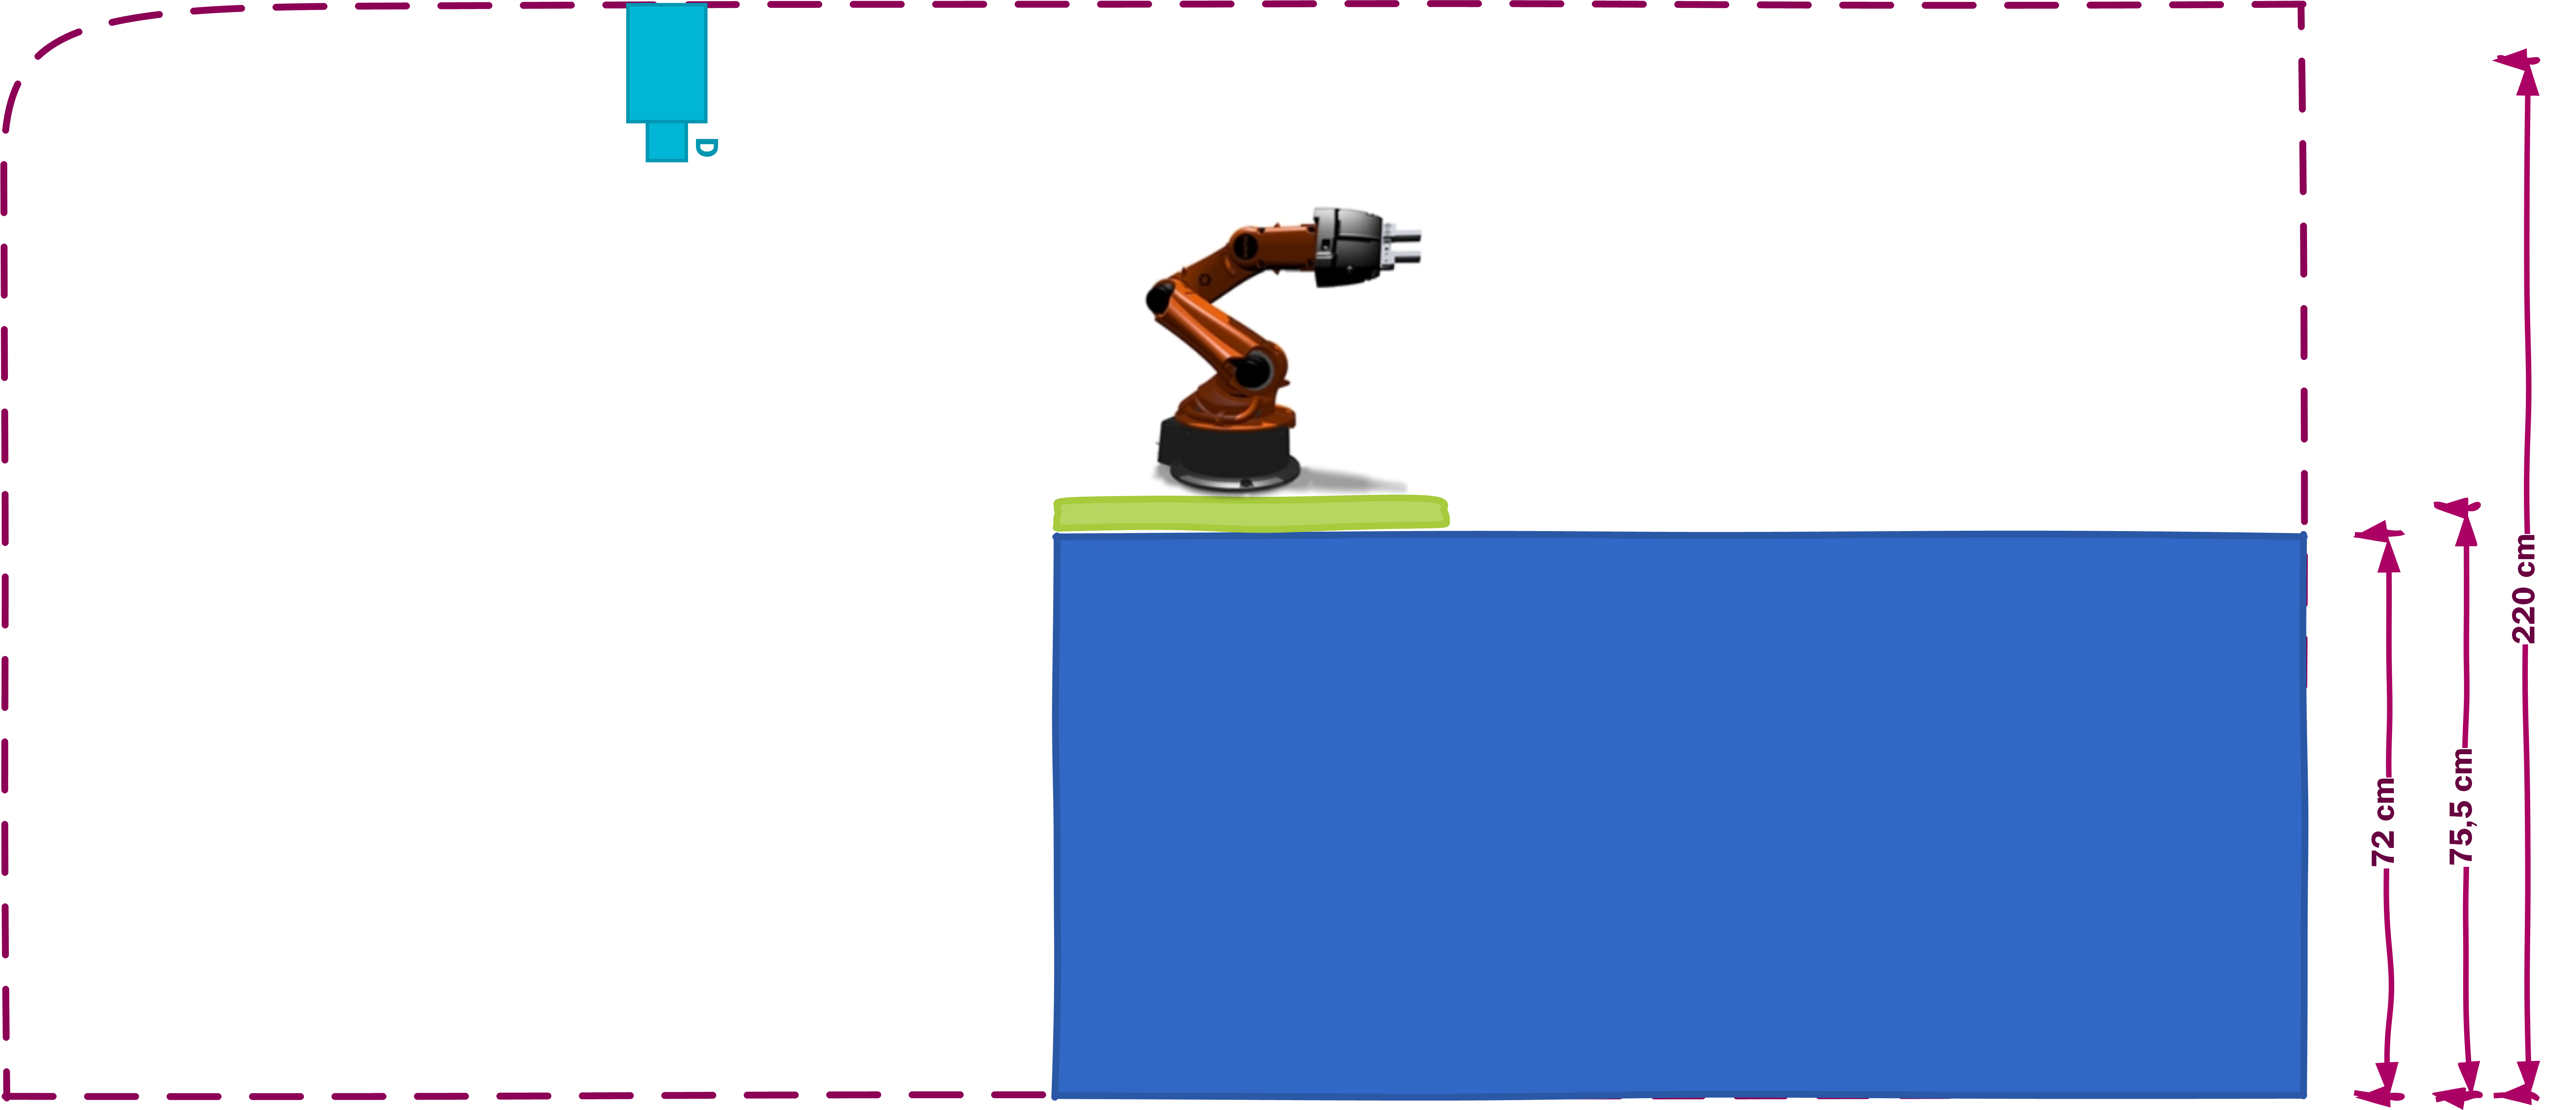
\includegraphics[scale=0.5]{fig/ZeichnungRaumH}   
  	\caption[Aufbau Teststand: Seitenansicht]{Der Aufbau}
  	\label{fig:basic-aufbau-teststandh}
  \end{figure}

\subsection{YouBot}
In dieser Arbeit werden zwei Roboter genutzt. Bei beiden handelt es sich um YouBots der Firma Kuka. Diese wurden 2010 erstmals auf der Automatica in München vorgestellt. Kuka ist ein deutscher Hersteller von Industrierobotern mit Sitz in Augsburg. Kuka hat aber auch Erfahrung im Bau von experimentellen Robotern wie etwas die Arme für Justin, einem Service-Roboter.

Die beiden YouBots unterscheiden sich beim Aufbau. YouBot 1 besteht aus einem Manipulator mit Gripper, YouBot 2 besteht aus Manipulator mit Gripper und mobiler Plattform mit omnidirektionalen Rollen. Zur besseren Unterscheidung und zur Lesbarkeit dieser Arbeit haben beide Roboter einen Namen bekommen. YouBot 1 entspricht dabei \textbf{Dummy}, YouBot 2 ist \textbf{Rose}. Im Weiteren Verlauf der Arbeit werden nur noch diese Namen genutzt um eine Verwechslung zu vermeiden.


\subsubsection{Manipulator}
 Die Roboterarme von Dummy und Rose sind eine offene kinematische Kette mit fünf Joints, die von der Basis aufsteigend nummeriert sind. An Joint 5 sind die Gripper montiert, diese bestehen aus zwei individuellen Fingern, die linear auf einer Achse bewegt werden können.

Joint 1 und Joint 5 sind zwei Drehgelenke um die Z-Achse, die bei ausgestreckter Haltung (Candle-Pose) parallel liegen. Joint 2, 3 und 4 sind Kippgelenke um die X-Achse, die immer parallel liegen. Durch diese Konstellation ergeben sich für den kompletten Arm fünf Freiheitsgrade (5-DOF). Durch die Einschränkung der Achsen auf die X- und Z-Achsen der einzelnen Joints ist ein seitlicher Griff bei $x_{base} = 0$ oder $y_{base} = 0$ nicht möglich. Die Höhe in Candle-Pose beträgt inklusiv Gripper 655mm. Die einzelnen Abstände lassen sich der Grafik \ref{fig:basic-aufbau-youbot-kinematik} entnehmen.

\begin{figure}[H]
	\centering
	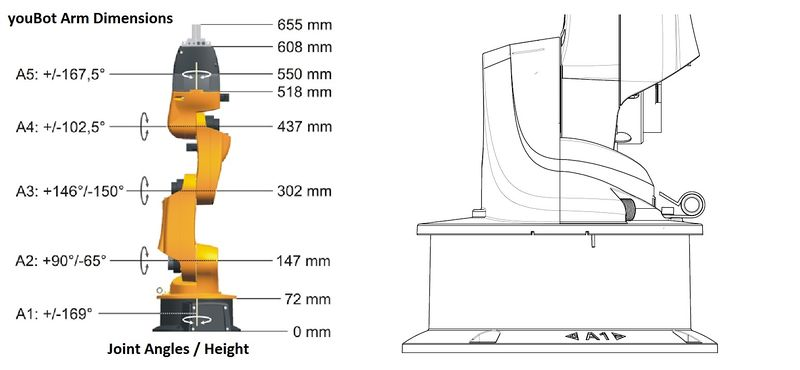
\includegraphics[scale=0.8]{fig/kukaarm_1}   
	\caption[YouBot Arm Kinematik]{YouBot Arm Kinematik. Links: Detaillierter Mechanismus mit Joint und Link Angaben. Rechts: Vergrößerte Darstellung der Basis. Bildquelle: \cite{monikaflorekjasinska2015}}
	\label{fig:basic-aufbau-youbot-kinematik}
\end{figure}



 
 Tabelle \ref{tab:basic-aufbau-youbot-joints} stellt noch einmal den Drehbereich aller Joints dar. Dabei sind neben Bezeichner auch die minimalen und maximalen Winkel, sowie die Winkelgeschwindigkeiten. Eine Besonderheit stellt Joint 3 dar, durch den Aufbau bedingt wurde die Achse innerhalb der Treiber gespiegelt, sodass die Winkel um den 0° Punkt gespiegelt wurden. In der Tabelle und den folgenden Zeichnungen ist diese Spiegelung nicht beachtet.
 
   \begin{table}[H]
   	\begin{tabular}{|c|c|c|}
   		\hline Bezeichnung & Max./Min. Winkel & Winkelgeschwindigkeit (rad / s) \\ 
   		\hline Joint 1 & $\pm$ 2.94 & $\frac{\pi}{2}$  \\ 
   		\hline Joint 2 & + $\frac{\pi}{2}$ / -1.13  & $\frac{\pi}{2}$ \\ 
   		\hline Joint 3 & +2.54 /-2.63 & $\frac{\pi}{2}$ \\ 
   		\hline Joint 4 & $\pm$1.78 & $\frac{\pi}{2}$ \\ 
   		\hline Joint 5 & $\pm$2.91 & $\frac{\pi}{2}$ \\ 
   		\hline 
   	\end{tabular}
   	\caption[YouBot Arm Joints]{YouBot Arm Joints. Quelle: \cite{monikaflorekjasinska2015}}
   	\label{tab:basic-aufbau-youbot-joints}
   \end{table}
   
   Der Arbeitsraum des YouBot Arms beschränkt sich durch die Joints. Die Grafiken \ref{fig:basic-aufbau-youbot-workspace} und \ref{fig:basic-aufbau-youbot-workspace-top} stellen den Arbeitsbereich eingeschränkt dar. Die Darstellung \ref{fig:basic-aufbau-youbot-workspace} zeigt mit Hilfe von Konturen die einzelnen Bahnen unter Beschränkung der Joints, sowie der End-Effektor Ausrichtung.  Die äußerste Kontur gibt die maximale Reichweite für den End-Effektor an. Die Z-Achse steht dabei orthogonal zur Tangente an der Konturposition. Abbildung \ref{fig:basic-aufbau-youbot-workspace-top} gibt eine Draufsicht auf den Arbeitsraum. Durch die Beschränkung von Joint 1 befindet sich ein toter Winkel im "Rücken" der Arms. Dieser kann durch einen Überschlag des ganzen Arm, insbesondere Joint 2 und 3, und einer 180 \textdegree Drehung von Joint 1 dennoch erreicht werden. Dies wird durch den linken Bereich in Abbildung \ref{fig:basic-aufbau-youbot-workspace} klar.
   
   
   \begin{figure}
   	\centering
   	\subfigure[YouBot Arm Arbeitsraum. Reichweite der einzelnen Gelenk und einzelne Abmessung der Links und Link-Offsets. Einheitslose Angaben sind in mm.]{%
   		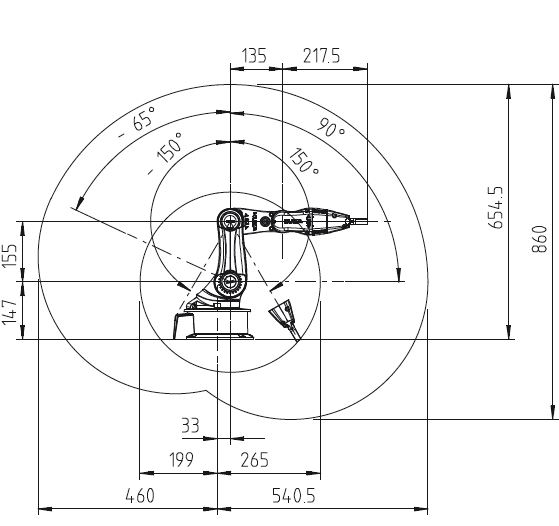
\includegraphics[scale=0.55]{fig/kukaarm_2}
   		\label{fig:basic-aufbau-youbot-workspace}}
   	\hfill
   	\subfigure[Draufsicht YouBot Arm Arbeitsraum.]{%
   		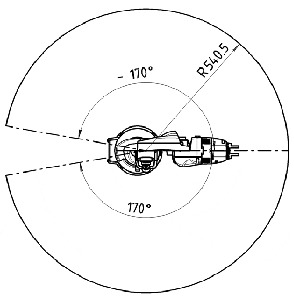
\includegraphics[scale=0.55]{fig/kukaarm_3}
   		\label{fig:basic-aufbau-youbot-workspace-top}}
   	\caption{Arbeitsraum YouBot. Bilderquelle:\cite{monikaflorekjasinska2015}}
   	\label{fig:basic-aufbau-youbot-workspace-full}
   \end{figure}

\subsubsection{Mobile Plattform}
Rose besitzt neben dem Arm noch eine mobile Plattform. Diese ist 590 mm lang, 380 mm breit und 140 mm hoch. Die Plattform hat vier Räder mit einem Durchmesser von 47.5 mm. Jedes Rad lässt sich getrennt ansteuern. Bei den Rädern handelt es sich um Mecanum-Räder, die eine Steuerung in alle Richtungen ermöglicht. Dazu sitzen auf jeder Felge sechs drehbare tonnenförmige Rollen die im Winkel von 45° zur Achse des Rades angebracht sind. Damit Omni-Direktionale Bewegungen möglich sind werden die Räder abwechselnd zum Nachbar auf +45° oder -45° angeordnet. Die minimale Geschwindigkeit der Plattform beträgt $0.01\frac{m}{s}$, die maximale  $0.8\frac{m}{s}$. Abbildung \ref{fig:basic-aufbau-youbot-base} zeigt den Aufbau und Abmessungen der Plattform. 

\begin{figure}[H]
	\centering
	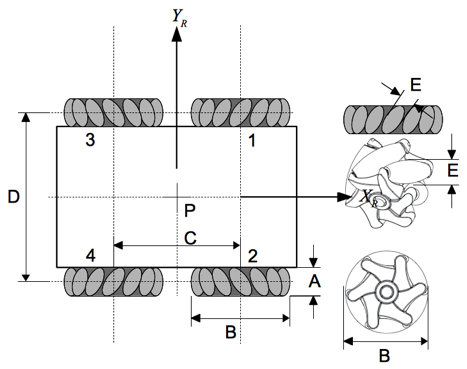
\includegraphics[scale=0.8]{fig/kukabase}   
	\caption[YouBot Base]{YouBot Base. A = 74.87 mm, B = 100 mm, C = 471 mm, D = 300.46 mm E = 28 mm. Die Bodenfreiheit der Plattform beträgt 20 mm. Bildquelle: \cite{monikaflorekjasinska2015}}
	\label{fig:basic-aufbau-youbot-base}
\end{figure}

Die Plattform von Rose ist modifiziert und besitzt eine Aufsatzplatte. Diese dient zur Montage zusätzlicher Sensoren und zur Schutz der Räder bei Kollisionen. Diese ist 600 mm lang und 396 mm breit. Durch die Abstandsbolzen und die Dicke der Platte (5 mm) erhöht sich die Plattform auf 150 mm (siehe Abbildung \ref{fig:basic-aufbau-youbot-base_side}).  

 \begin{figure}[H]
 	\centering
 	\subfigure[Seitenansicht mobile Plattform mit Sensorplatte]{%
 		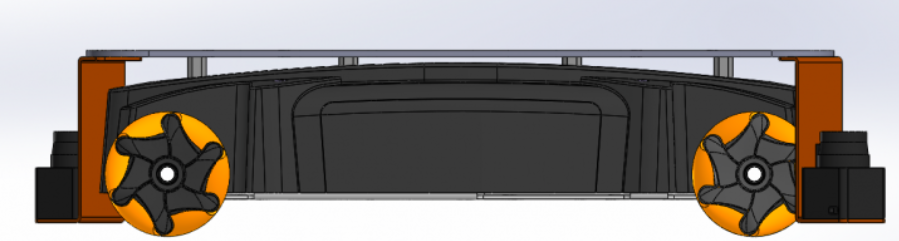
\includegraphics[scale=0.55]{fig/base2}
 		\label{fig:basic-aufbau-youbot-base_side}}
 	\subfigure[Draufsicht mobile Plattform mit Sensorplatte]{%
 		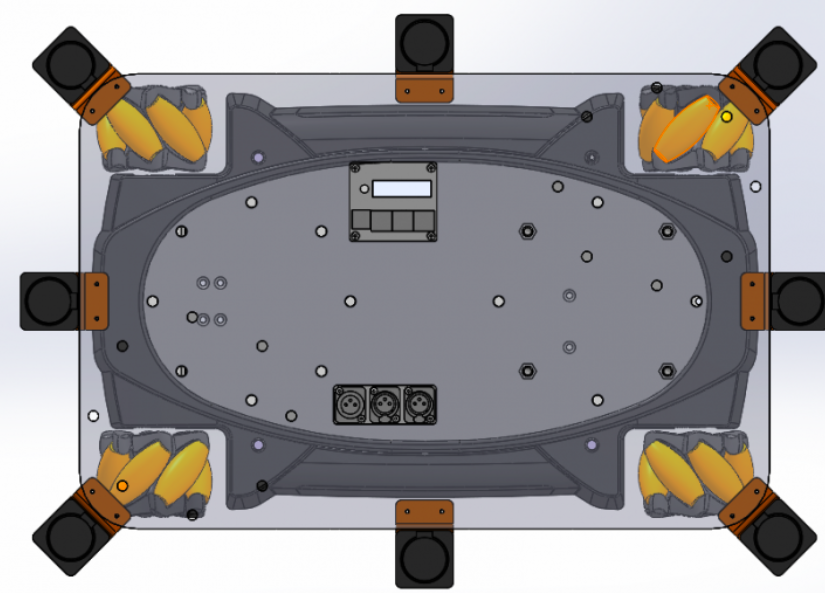
\includegraphics[scale=0.55]{fig/base3}
 		\label{fig:basic-aufbau-youbot-base-top}}
 	\caption{Mobile YouBot Plattform mit Sensorplatte. Bilderquelle:\cite{kuka2015}}
 	\label{fig:basic-aufbau-youbot-base-full}
 \end{figure}

\subsubsection{Rechner}
Für die Rechenleistung der beiden Roboter sorgen neben den verbauten, eingebetteten Boards zwei Computer mit Linux Betriebssystemen.
Der für Rose zuständige PC ist ein Mini-ITX und in der mobilen Plattform eingebaut. Dieser läuft mit einem Intel Atom D510 Dual Core mit 1.66 GHz als CPU und 2 GB DDR2 RAM. Als Festplattensystem ist eine 32 GB SSD verbaut. Der Rechner stellt einige IO-Schnittstellen zur Verfügung: sechs USB 2.0, ein VGA und zwei LAN Anschlüsse sind nutzbar. Dabei ist ein LAN Anschluss für den Ethercat-Anschluss der Plattform belegt. Diese wiederum bringt nochmal zwei LAN Anschlüsse mit. Der Rechner für Dummy ist ein BLALBLA %TODO Dummy PC

Weitere Details zu den Armen, der Plattform oder den Rechnern befindet sich im Anhang.%TODO Anhang

\subsection{Sensoren}
Für die Erkennung von Objekten und der Positionierung im Raum sind mehrere Sensoren nötig. In dieser Arbeit wird dabei auf das Kamerasystem Asus XTion Pro Live und auf einen Laserscanner Hokuyo URG-04LX-UG01 zurückgegriffen.

\subsubsection{Asus XTion Pro}
Die XTion Pro ist ein Tiefenkamerasystem von Asus. Es besteht aus einer RGB-Kamera, einer Tiefen-Kamera und zwei Mikrophonen. Die Kamera wurde von Prime Sense entwickelt und ist eine umgelabelte Microsoft Kinect. Die XTion ist kleiner und leichter als die Kinect und damit besser für die Robotik geeignet. Angeschlossen wird die XTion mit einem USB Kabel und betrieben mit dem ROS Paket OpenNI2. Das Sichtfeld der Kamera beträgt Horizontal 58\textdegree, 45\textdegree Vertikal und 70\textdegree Diagonal. Die Auflösung der Tiefenkamera beträgt bei 30 Frames pro Sekunde 640x480 und bei 60 FPS 320x240. Die Auflösung des RGB-Bildes 1280x1024. Die nutzbare Distanz der Tiefenkamera beträgt zwischen 800 mm und 3500 mm. Diese Distanz schränkt die Nutzbarkeit der Kamera ein, so ist sie nicht für eine visuelle Unterstützung der Gripper geeignet, wenn sie an diesen montiert ist.


\subsubsection{Hokuyo URG-04LX-UG01}
\subsubsection{Netzwerk}
